\documentclass[12pt, A4]{article}
\usepackage[utf8]{inputenc}
\usepackage{geometry}
\geometry{
	a4paper,
	left=15mm,
	right=15mm,
	top=25mm,
	bottom=25mm
}
\usepackage{graphicx}
\graphicspath{ {./images/} }
\usepackage{amsmath}
\usepackage{amsfonts}
\usepackage{amssymb}
\usepackage{hyperref}
\hypersetup{
	colorlinks=true,
	linkcolor=black,
	filecolor=magenta,      
	urlcolor=cyan,
	pdfpagemode=FullScreen,
}

\usepackage{amsthm}
\makeatletter
\newtheorem*{remark}{Remark}

\renewcommand{\theenumi}{\roman{enumi}}

\newcommand{\indep}{\perp \!\!\! \perp}

\newcommand{\sq}{$\square$}
\newcommand{\rmk}{$\surd$}
\newcommand{\trick}{$\bigstar$}
\newcommand{\N}{\mathbb{N}}
\newcommand{\R}{\mathbb{R}}
\newcommand{\Z}{\mathbb{Z}}
\newcommand{\Q}{\mathbb{Q}}
\newcommand{\U}{\mathcal{U}}
\newcommand{\V}{\mathcal{V}}
\newcommand{\A}{\mathcal{A}}
\newcommand{\B}{\mathcal{B}}
\newcommand{\C}{\mathcal{C}}
\newcommand{\G}{\mathcal{G}}
\newcommand{\F}{\mathcal{F}}
\newcommand{\LL}{\mathcal{L}}
\newcommand{\open}{\underset{open}{\subset}}
\newcommand{\closed}{\underset{closed}{\subset}}
\newcommand{\subsp}{\underset{subsp}{\subset}}
\newcommand{\seq}{\underset{seq}{\subset}}
\newcommand{\cl}{\overline}
\newcommand{\diff}{\,\backslash\,}
\newcommand{\union}{\,\cup\,}
\newcommand{\intersect}{\,\cap\,}
\newcommand{\exist}{\exists\,}
\newcommand{\convp}{\overset{P}{\rightarrow}}
\newcommand{\convd}{\overset{D}{\rightarrow}}
\newcommand{\foranyn}{\quad \forall \, n\in \N}

\begin{document}
\begin{titlepage}
	\begin{center}
		\vspace*{5cm}
		\textbf{\Large Probability theory \MakeUppercase{\romannumeral 2} Assignment 2}
		\\
		\vspace{1.5cm}
		\textbf{2021-21116 Taeyoung Chang}
		\vfill
		Exercises \\ Section 4.2 Martinagles, Almost Sure Convergence \\ Section 4.3 Examples \\ Section 4.4 Doob's Inequality, Convergence in $L^p$ 
	
		\vspace*{3cm}
		\thispagestyle{empty}
	\end{center}
\end{titlepage}

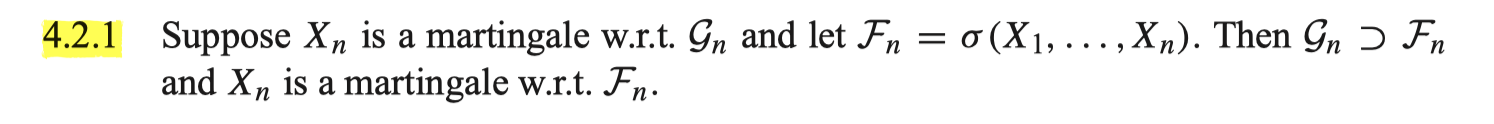
\includegraphics[width=17cm]{Exer4.2.1.png}

\begin{proof}
    Since $X_n$ is a martingale w.r.t $\G_n$ , $X_n$ is integrable. Also, $X_n\in \G_n\foranyn$ . Define a sequence of collections $\{\A_n\}_n$ as
    $$
        \A_n=\{(X_j\in B) : j=1, \cdots, n \; \text{and}\; B\in \B(\R)\}
    $$
    Then we have $\F_n=\sigma(\A_n)\foranyn$ . Take any $B\in \B(\R)$ and $j\in \{1, \cdots, n\}$ . Since $X_n\in \G_n$ , we have $(X_j\in B)\in \G_j\subset \G_n$ . It implies that $\A_n\subset \G_n\foranyn$ . Furthermore , since $\G_n$ is a $\sigma$-field, we get $\sigma(\A_n)\subset \G_n\foranyn$ . Therefore $\F_n\subset \G_n \foranyn$ . \\  
    Now we should show that $X_n$ is a martingale w.r.t $\F_n$ . As we said before, $X_n$ is integrable. Also, $X_n\in \F_n\foranyn$ by the definition of $\F_n$. Finally, $E[X_{n+1}|\F_n]=X_n \foranyn$ since
    \begin{align*}
        E[X_{n+1}|\F_n] &= E[E[X_{n+1}|\G_n]\big|\F_n] \quad \because \;\F_n\subset \G_n \quad \text{smoothing property} \\
        &= E[X_n|\F_n] \quad \because \; X_n\; \text{is martingale w.r.t} \; \G_n \\
        &= X_n \quad \because \; X_n\in \F_n
    \end{align*}
    Thus, $X_n$ is a martingale w.r.t $\F_n$
\end{proof}

\begin{remark}
    If $X_n$ is a martingale then  $\F_n$ defined by $\F_n=\sigma(X_1, \cdots, X_n)$ is the smallest filtration that makes $X_n$ a martingale.
\end{remark}

\vspace{1cm}
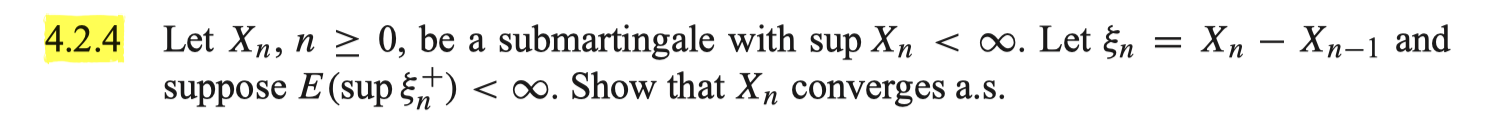
\includegraphics[width=17cm]{Exer4.2.4.png}

\begin{proof}
    Take $M\in \N$ . Define $N=\inf\{n\in \N\union \{0\} : X_n>M \}$ . Then $N$ is a stopping time.
    $$\because (N=n)=(X_0\leq M)\intersect \cdots \intersect (X_{n-1}\leq M)\intersect (X_n>M)\in \F_n \foranyn$$
    Consider $X_{N\wedge n}$ . Since $X_n$ is a martingale and $N$ is a stopping time, $X_{N\wedge n}$ is also a submartingale. \\
    \begin{enumerate}
        \item If $n<N$ \\ $X_{N\wedge n}=X_n$ and $X_n\leq M$ . Also $X_n^+\leq M$
        \item Else, if $n\geq N$ \\ $X_{N\wedge n}=X_N>M$ . Note that $X_{N-1}\leq M$ and $\xi_N=X_N-X_{N-1}$ . Hence we have \\ $X_N=X_{N-1}+\xi_N \leq M+\xi_N^+\leq M+\sup_n \xi_n^+\foranyn$ and also $X_N^+\leq M+\sup_n \xi_n^+\foranyn$
    \end{enumerate}
    Combining two cases , we have $X_{N\wedge n}^+\leq M+\sup_n \xi_n^+\foranyn$ . \\Taking expectation, we have $E[X_{N\wedge n}^+]\leq M+E[\sup_n \xi_n^+]\foranyn$ . \\By taking supremum, we get $\sup_n E[X_{N\wedge n}^+]\leq M+E[\sup_n \xi_n^+]$ \\ Since $E[\sup_n \xi_n^+]<\infty$ by assumption, we have $\sup_n E[X_{N\wedge n}^+]<\infty$ . By the submartingale convergence theorem, $X_{N\wedge n}$ converges $a.s.$ \\ Note that if $N=\infty$ then $X_{N\wedge n}=X_n\foranyn$ . Hence $X_n$ converges $a.s.$ on $(N=\infty)$ \\ We have taken arbitrary $M\in \N$ for defining a stopping time $N$. Hence we can write it as $N_M$ to emphasize that it depends on the value of $M$ . Then for each $M\in \N$, we have $$(N_M=\infty) = (X_n\leq M\foranyn)= \Big(\sup_{n}X_n\leq M\Big) $$ Therefore $P\Big(\sup_{n}X_n\leq M\Big)= P(N_M=\infty) \quad \forall \; M\in \N$ . Observe that $\Big(\sup_{n}X_n\leq M\Big)$ is increasing sequence of events w.r.t $M$ . i.e.  $\Big(\sup_{n}X_n\leq M\Big)\subset \Big(\sup_{n}X_n\leq M+1\Big)\quad \forall \; M\in \N$ . Thus $(N_M=\infty)$ is also increasing sequence of events w.r.t $M$ \\ By assumption $\sup_n X_n<\infty\;\, a.s.$ , $$1=P\Big(\sup_{n}X_n<\infty \Big)=P\Big(\bigcup_{M\in \N}\big(\sup_{n}X_n\leq M \big)\Big)=\lim_{M\rightarrow \infty} P\Big(\sup_{n}X_n\leq M\Big)$$
    due to continuity from below of probability measure. Combining the results above, we have $$1=\lim_{M\rightarrow \infty}P(N_M=\infty)=P\Big(\bigcup_{M\in \N}\big( N_M=\infty\big)\Big) $$ Let $C=\Big(\bigcup_{M\in \N}\big( N_M=\infty\big)\Big)$ . Since $X_n$ converges $a.s.$ on $(N_M=\infty)$ for every $M\in \N$ , we have $X_n$ converges $a.s.$ on $C$ with $P(C)=1$ . Therefore $X_n$ converges $a.s.$
\end{proof}
\vspace{1cm}

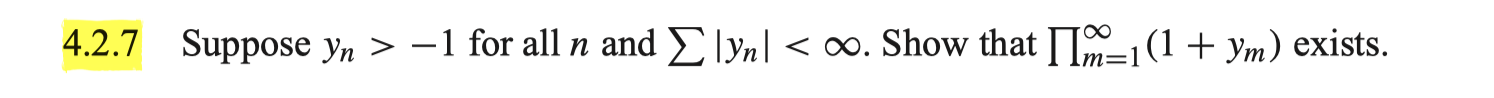
\includegraphics[width=17cm]{Exer4.2.7.png}
\begin{figure}[h]
    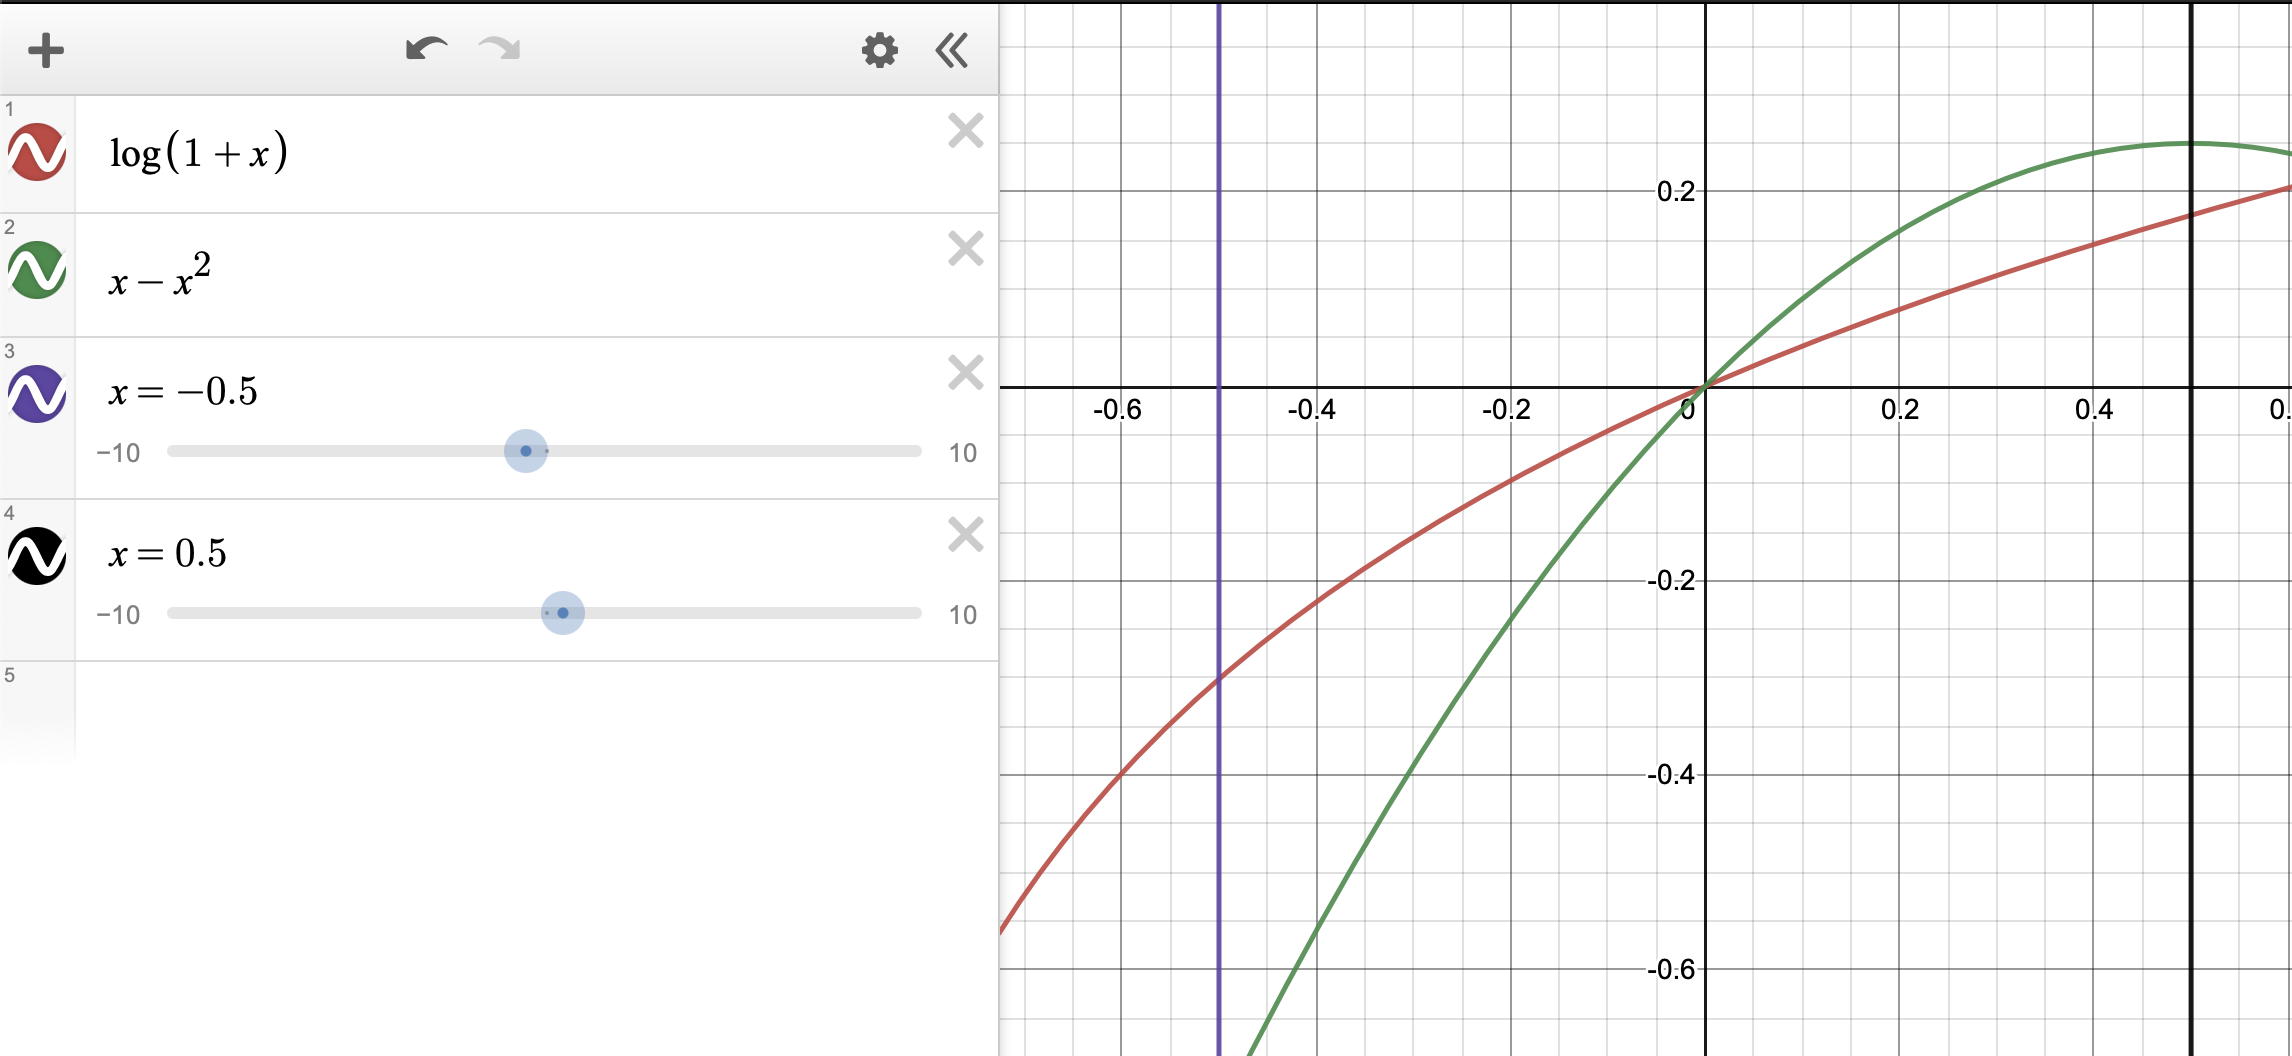
\includegraphics[width=17cm]{Graph4.2.7.png}
\end{figure}
\begin{proof}
    We shall use the result $|\log(1+x)|\leq |x-x^2| \quad \forall \; |x|\leq \frac{1}{2}\quad \cdots (*)$ by the visual result of graphing device (Desmos) . \\ From the assumption $\sum_n |y_n|<\infty$ , we have $y_n\rightarrow 0$ as $n\rightarrow \infty$ . Thus $\exists \;M\in \N\;$ s.t. \\$|y_n|\leq \frac{1}{2}\quad \forall\; n\geq M$ which implies $y_n^2\leq \frac{1}{4} \quad \forall \; n\geq M$ . Since $\sum_n \big(\frac{1}{4}\big)^n$ converges , $\sum_n y_n^2$ also converges by the comparison test. Now take $N\in \N$ s.t. $N\geq M$ and observe that
    $$\Big|\sum_{n>N} \log(1+y_n)\Big|\leq \sum_{n>N}|\log(1+y_n)|\leq \sum_{n>N}|y_n-y_n^2|\leq \sum_{n>N}|y_n| + \sum_{n>N}y_n^2\longrightarrow 0\quad \text{as} \quad N\rightarrow \infty$$
    The second inequality comes from the two fact : $|y_n|\leq \frac{1}{2} \quad \forall \; n\geq M$ and the inequality $(*)$ . The convergence to zero is derived from the fact that $\sum_n |y_n|$ and $\sum_n y_n^2$ are both convergent series and the tail part of the convergent series tends to zero. \\
    Therefore $\sum_n \log(1+y_n)$ converges to a finite number and $\prod_n (1+y_n)=\exp(\sum_n\log(1+y_n))$ also converges to a finite number 
\end{proof}
\vspace{1cm}

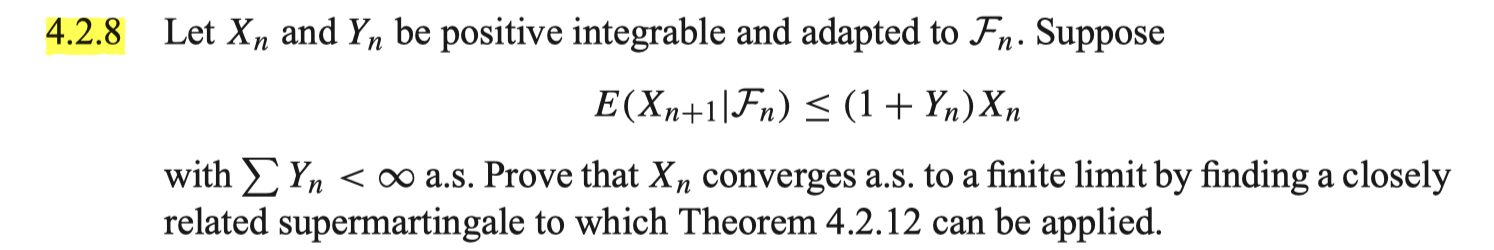
\includegraphics[width=17cm]{Exer4.2.8.png}
\begin{proof}
    We shall define a nonnegative supermartingale to utilize supermartingale convergence thm. $$W_n:=\frac{X_n}{\prod_{m=1}^{n-1}(1+Y_m)} $$
    Since $X_n$ and $Y_n$ are positive , $W_n$ is also positive. Also , $X_n\in \F_n$ and $\prod_{m=1}^{n-1}(1+Y_m)\in \F_{n-1}\subset \F_n$ , we have $W_n\in \F_n \foranyn$ . Note that $(1+Y_n)>1$ so that $\prod_{m=1}^n (1+Y_m)>1 \foranyn$ 
    $$E(W_n)= E\Big[\frac{X_n}{\prod_{m=1}^{n-1}(1+Y_m)}\Big]\leq E[X_n]<\infty \foranyn$$ The last inequality $E(X_n)<\infty$ comes from the assumption that $X_n$ is integrable. Thus $W_n$ is integrable. To show $W_n$ is a supermartingale, it suffices to show that $E[W_{n+1}|\F_n]\leq W_n$
    \begin{align*}
        E[W_{n+1}|\F_n] &= E\Big[\frac{X_{n+1}}{\prod_{m=1}^{n}(1+Y_m)}\big|\F_n\Big] \\
        &= \frac{1}{\prod_{m=1}^n(1+Y_m)}E[X_{n+1}|\F_n] \quad \because \; \frac{1}{\prod_{m=1}^n(1+Y_m)}\in \F_n \\ &\leq \frac{1}{\prod_{m=1}^n(1+Y_m)}(1+Y_n)X_n \quad \because \; \text{By assumption}\quad E[X_{n+1}|\F_n]\leq (1+Y_n)X_n \\ 
        &=\frac{1}{\prod_{m=1}^{n-1}(1+Y_m)}X_n = W_n
    \end{align*}
    Therefore, $W_n$ is a nonnegative supermartingale. By supermartingale convergence thm , \\$W_n\rightarrow W\;\,a.s.$ for some integrable r.v. $W$. Note that $$X_n=W_n \prod_{m=1}^{n-1}(1+Y_m)$$ Since $Y_n>0$ and $\sum_n Y_n<\infty\;\,a.s.$ by the assumption, we can apply the result of the previous exercise so that $\prod_n (1+Y_n)$ converges $a.s.$ . In other words,  $\prod_n (1+Y_n)\rightarrow Z\;\,a.s.$ for some r.v. $Z$ . Then we can conclude that $X_n\rightarrow WZ\;\,a.s.$ . Note that $Z$ is finite by the result of the previous exercise and $W$ is finite $a.s.$ since it is nonnegative and integrable. Hence $WZ$ is finite $a.s.$
\end{proof}
\vspace{1cm}

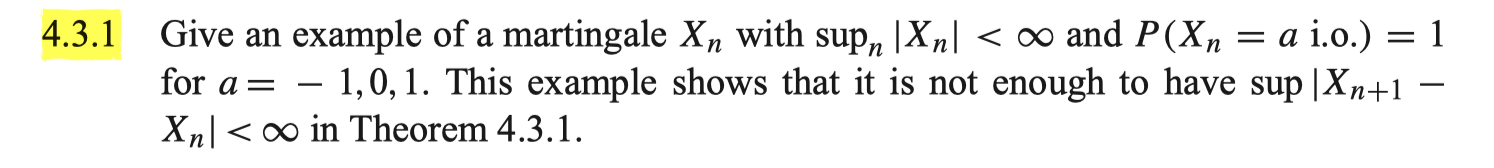
\includegraphics[width=17cm]{Exer4.3.1.png}
\begin{proof}
    Let $\{U_n\}_n$ be i.i.d random sequence with $U_1\sim Unif(0,1)$ and $\F_n:=\sigma(U_1, \cdots, U_n)$ \\ Let $X_0=0$ and define $X_n$ for each $n\in \N$ as below :
    \begin{equation*} 
        X_{n+1} =
        \begin{cases}
            \begin{cases}
                1 & \text{if}\; U_{n+1}\geq \frac{1}{2} \\
                -1 & \text{if}\; U_{n+1}< \frac{1}{2}
            \end{cases}
            & \text{if}\; X_n =0  \\
            \begin{cases}
                0 & \text{if}\; U_{n+1}\geq \frac{1}{n^2} \\
                n^2 X_n & \text{if}\; U_{n+1}< \frac{1}{n^2}
            \end{cases} & \text{if}\; X_n\neq 0
        \end{cases}
    \end{equation*}
    Note that $P(U_n<\frac{1}{n^2})=\frac{1}{n^2}\foranyn$ and $\sum_n P(U_n<\frac{1}{n^2})= \sum_n \frac{1}{n^2}<\infty$ . By Borel Cantelli lemma, this implies that $P(U_{n+1}<\frac{1}{n^2}\;\,i.o.)=0$ In other words, $$ P(U_{n+1}\geq \frac{1}{n^2}\;\,\text{all but finitely many n})=1$$
    Let $B=(U_{n+1}\geq \frac{1}{n^2}\;\,\text{all but finitely many n})$ . Then $P(B)=1$ and for each $\omega\in B$ , there is large enough $N$ s.t. sequence $X_N, X_{N+1}, X_{N+2}, \cdots$ is given by $0,\pm1, 0, \pm1, \cdots$ . \\ Hence $\omega \in (X_n=1\;\,i.o.)\intersect (X_n=-1\;\,i.o.)\intersect (X_n=0\;\,i.o.)$ whenever $\omega\in B$ . Since $P(B)=1$, we have $P(X_n=a \;\,i.o.)=1$ for $a=-1,1,0$ \\ Also, since $|X_n|\leq (n!)^2 \foranyn$ and $|X_n|\leq 1$ for large enough $n\;\,a.s.$ we have $\sup_n|X_n|<\infty$ . By this , $X_n$ is integrable. Also $X_n\in \F_n$ . To show $X_n$ is a martingale , it suffices to show that $E[X_{n+1}|\F_n]=X_n$
    \begin{align*}
        E[X_{n+1}|\F_n] &=E[X_{n+1}I(X_n=0)+X_{n+1}I(X_n\neq 0)|\F_n] \\
        &= E[X_{n+1}I(X_n=0)|\F_n] +E[X_{n+1}I(X_n\neq 0)|\F_n] \\
        &= I(X_n=0)E[X_{n+1}|\F_n] + I(X_n\neq 0)E[X_{n+1}|\F_n] \\
        &= I(X_n=0)\{\frac{1}{2}\cdot 1+\frac{1}{2}\cdot (-1)\} + I(X_n\neq 0)\Big\{(1-\frac{1}{n^2})\cdot 0 + \frac{1}{n^2}\cdot n^2X_n\Big\} \\ 
        &= 0\cdot I(X_n=0) + X_n\cdot I(X_n\neq 0) = X_n
    \end{align*}
    Therefore $X_n$ is a martingale w.r.t $\F_n$
\end{proof}
\vspace{1cm}

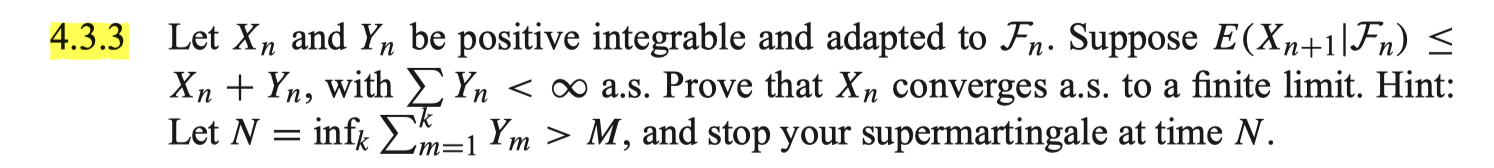
\includegraphics[width=17cm]{Exer4.3.3.png}
\begin{proof}
    We want to define a supermartingale. Define $W_n$ as below :
    $$
        W_n := X_n-\sum_{m=1}^{n-1} Y_m \quad \foranyn
    $$
    We shall show that $W_n$ is a supermartingale w.r.t $\F_n$ .\\ First, since $X_n\in \F_n$ and $\sum_{m=1}^{n-1}Y_m\in \F_{n-1}\subset \F_n$ , we have $W_n\in \F_n\foranyn$ \\ Second, $E|W_n|\leq E|X_n|+\sum_{m=1}^{n-1}E|Y_m|$ and $X_n$ , $Y_n$ are all integrable so that $E|W_n|<\infty$ \\
    For showing $W_n$ is a supermartingale , it suffices to show that $E[W_{n+1}|\F_n]\leq W_n$
    \begin{align*}
        E[W_{n+1}|\F_n] &= E\Big[X_{n+1}-\sum_{m=1}^n Y_m \big|\F_n\Big] = E[X_{n+1}|\F_n]-\sum_{m=1}^n Y_m \\ &\leq X_n+Y_n - \sum_{m=1}^n Y_m \quad \because \; E[X_{n+1}|\F_n]\leq X_n+Y_n \quad \text{by assumption} \\ &= X_n -\sum_{m=1}^{n-1}Y_m = W_n
    \end{align*}
    Therefore, $W_n$ is a supermartingale. \\ Take $M\in \N$ and define $N=\inf\{n\in \N : \sum_{m=1}^n Y_m>M\}$ . Then $N$ is a stopping time. 
    $$ \because (N=n)= (\sum_{m=1}^{n-1}Y_m \leq M)\intersect (\sum_{m=1}^n Y_m >M) \in \F_n \foranyn$$
    Since $W_n$ is a supermartingale and $N$ is a stopping time, $W_{N\wedge n}$ is a supermartingale. \\
    \begin{align*}
        W_{N\wedge n } &=X_{N\wedge n} - \sum_{m=1}^{(N\wedge n) -1}Y_m \\ 
        &\geq X_{N\wedge n}-M \quad \because \sum_{m=1}^{(N\wedge n)-1} Y_m \leq \sum_{m=1}^{N-1}Y_m\leq M \\
        W_{N\wedge n}+M &\geq X_{N\wedge n}>0
    \end{align*}
    We have used the assumption that $X_n$ and $Y_n$ are positive.\\ Thus $W_{N\wedge n}+M$ is nonnegative supermartingale. By supermartingale convergence thm, $W_{N\wedge n}+M$ converges $a.s.$ to an integrable random variable. It implies that $W_{N\wedge n}\rightarrow W\;\,a.s.$ for some integrable r.v. $W$ . Note that if $N=\infty$ then $W_{N\wedge n}=W_n\foranyn$ so that $W_n\rightarrow W\;\,a.s.$ on $(N=\infty)$ \\
    We have taken arbitrary $M\in \N$ for defining a stopping time $N$. Hence we can write it as $N_M$ to emphasize that it depends on the value of $M$ . Then for each $M\in \N$, we have $$(N_M=\infty) = (\sum_{m=1}^n Y_m\leq M \foranyn)= \Big(\sum_{n}Y_n\leq M\Big) $$ Therefore $P\Big(\sum_{n}Y_n\leq M\Big)= P(N_M=\infty) \quad \forall \; M\in \N$ . Observe that $\Big(\sum_{n}Y_n\leq M\Big)$ is increasing sequence of events w.r.t $M$ . i.e.  $\Big(\sum_{n}Y_n\leq M\Big)\subset \Big(\sum_{n}Y_n\leq M+1\Big)\quad \forall \; M\in \N$ . Thus $(N_M=\infty)$ is also increasing sequence of events w.r.t $M$ \\ By assumption $\sum_n Y_n<\infty\;\, a.s.$ , $$1=P\Big(\sum_n Y_n<\infty \Big)=P\Big(\bigcup_{M\in \N}\big(\sum_n Y_n\leq M \big)\Big)=\lim_{M\rightarrow \infty} P\Big(\sum_n Y_n\leq M\Big)$$
    due to continuity from below of probability measure. Combining the results above, we have $$1=\lim_{M\rightarrow \infty}P(N_M=\infty)=P\Big(\bigcup_{M\in \N}\big( N_M=\infty\big)\Big) $$ Let $C=\Big(\bigcup_{M\in \N}\big( N_M=\infty\big)\Big)$ . Since $W_n\rightarrow W\;\, a.s.$ on $(N_M=\infty)$ for every $M\in \N$ , we have $W_n\rightarrow W\;\,a.s.$ on $C$ with $P(C)=1$ . Therefore $W_n\rightarrow W\;\,a.s.$ with $W$ being integrable. \\ Since $X_n= W_n+\sum_{m=1}^{n-1} Y_m$ , $X_n\rightarrow X\;\,a.s.$ where $X=W+\sum_n Y_n$ with $W$ and $\sum_n Y_n$ being finite $a.s.$ . Therefore $X_n$ converges $a.s.$ to a finite limit $X$
\end{proof}
\vspace{1cm}

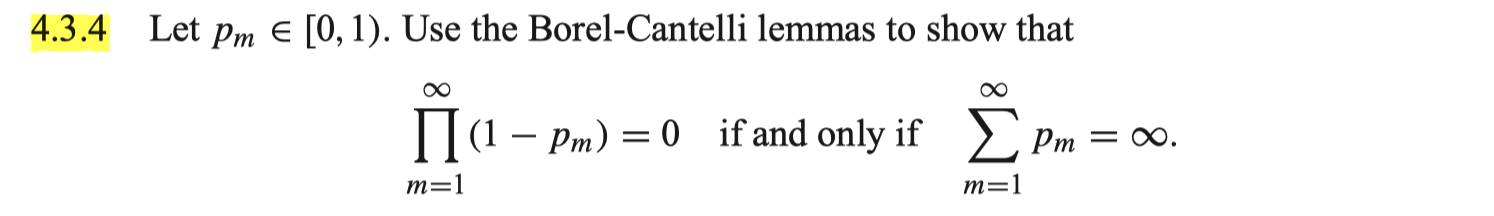
\includegraphics[width=17cm]{Exer4.3.4.png}
\begin{proof}
    Define a random sequence $\{X_n\}_n$ such that $X_n\overset{ind}{\sim} \text{Bern}(p_n)\foranyn$ . Using this random sequence, we can write that $$\prod_n (1-p_n) = P(X_n=0\foranyn) $$ 
    $(\Leftarrow)$ Suppose $\sum_n p_n=\infty$ . Then $\sum_n P(X_n=1)=\infty$ . Since $X_n$'s are independent, we can apply Borel Cantelli lemma so that $P(X_n=1\;\,i.o.)=1$ . Thus $P(X_n=0 \;\text{all but finitely many} \;n)=0$ . \\ Since $(X_n=0\foranyn)\subset (X_n=0 \;\text{all but finitely many} \;n)$ , we have $P(X_n=0 \foranyn)=0$ Therefore $\prod_n (1-p_n)=0$ \\
    $(\Rightarrow)$ Suppose $\sum_n p_n<\infty$ . Since the tail part of the convergent series tends to zero, we have large $N$ s.t. $\sum_{n>N} p_n <1$ so that $1-\sum_{n>N}p_n>0$
    \begin{align*}
        P(X_n=0 \quad\forall \; n>N) &= P\Big(\bigcap_{n>N}(X_n=0)\Big)= 1- P\Big(\bigcup_{n>N}(X_n=1)\Big) \\ &\geq 1-\sum_{n>N}P(X_n=1)=1-\sum_{n>N}p_n>0 \\
        P(X_n=0\foranyn) &= P(X_1=0)P(X_2=0)\cdots P(X_N=0)P(X_n=0\quad \forall\; n>N) \\
        &= (1-p_1)(1-p_2)\cdots(1-p_N)P(X_n=0\quad \forall\; n>N)>0 \quad \because p_n<1\;\forall\;n\; \text{is assumed}
    \end{align*}
    Thus $\prod_n (1-p_n)>0$ . As a result, $\sum_n p_n<\infty$ implies $\prod_n (1-p_n)>0$ . By contrapositive, we have the right direction proved.
\end{proof}
\begin{remark}
    Notice that for the left direction, we have not taken advantage of assumption $p_n<1 \quad \forall\; n$
\end{remark}
\vspace{1cm}

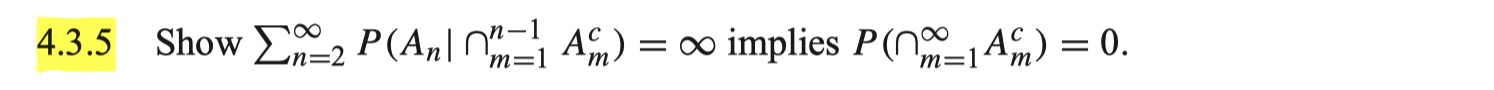
\includegraphics[width=17cm]{Exer4.3.5.png}
\begin{proof}
    Define $p_1=P(A_1)$ and $p_n=P(A_n|\bigcap_{m=1}^{n-1}A_m^C)\foranyn$ . \\By assumption, we have $\sum_n p_n=\infty$ . From the previous exercise, we get $\prod_n (1-p_n)=0\quad\cdots (*)$\\ $1-p_1=P(A_1^C)$ . What about $1-p_n$ for each $n>1$ ?
    \begin{align*}
        1-p_n &=1-P\Big(A_n\big|\bigcap_{m=1}^{n-1}A_m^C\Big) = 1- E\Big[I_{A_n}\big |\bigcap_{m=1}^{n-1}A_m^C \Big] =P(A_n^c \big | \bigcap_{m=1}^{n-1}A_m^C\Big) \\
        &= E\Big[1-I_{A_n} \big| \bigcap_{m=1}^{n-1}A_m^C \Big] = E\Big[I_{A_n^C}\big| \bigcap_{m=1}^{n-1}A_m^C\Big]=P\Big(A_n^c \big | \bigcap_{m=1}^{n-1}A_m^C\Big) =\frac{P\Big(\bigcap_{m=1}^{n}A_m^C\Big)}{P\Big(\bigcap_{m=1}^{n-1}A_m^C\Big)}
    \end{align*}
    Therefore, for each $n\in \N$, we can calculate $\sum_{m=1}^n (1-p_m)$ as below :
    $$\prod_{m=1}^n (1-p_m)=P(A_1^C)\frac{P(A_1^C\intersect A_2^C)}{P(A_1^C)}\frac{P(A_1^C\intersect A_2^C \intersect A_3^C)}{P(A_1^C\intersect A_2^C)}\cdots \frac{P\big(\bigcap_{m=1}^{n}A_m^C\big)}{P\big(\bigcap_{m=1}^{n-1}A_m^C\big)}=P\big(\bigcap_{m=1}^{n}A_m^C\big) $$
    Therefore, using continuity from above of probability measure , we have
    $$\prod_n (1-p_n)=\lim_{n\rightarrow \infty}\prod_{m=1}^n (1-p_m)=\lim_{n\rightarrow \infty}P\big(\bigcap_{m=1}^{n}A_m^C\big)=P\big(\bigcap_n A_n^C\big) $$  
    By $(*)$ above, we have $P\big(\bigcap_n A_n^C\big)=0$
\end{proof}
\vspace{1cm}

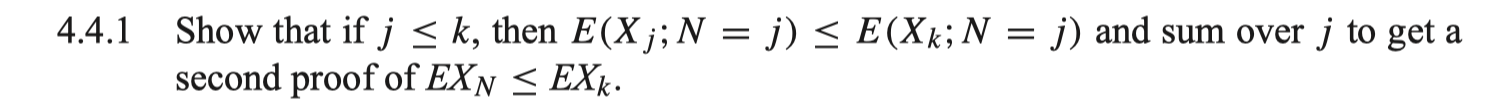
\includegraphics[width=17cm]{Exer4.4.1.png}
\begin{proof}
    Assume $X_n$ is a submartingale and $N$ is a stopping time w.r.t a filtration $\F_n$ . Suppose $N\leq k\;\,a.s.$ for some $k\in \N$ . Then $$ X_N=\sum_{j=0}^k X_j I(N=j)\;\,a.s.$$
    We shall claim that $$ E[X_j I(N=j)]\leq E[X_k I(N=j)]\quad \forall\; j\leq k$$
    Choose $j\leq k$ . Since $X_n$ is a submartingale , $X_j\leq E[X_k |\F_j]$ holds true. For $A_j\in \F_j$ ,
    \begin{align*}
        E[X_jI_{A_j}]&= \int_{A_j}X_j \, dP \leq \int_{A_j} E[X_k|\F_j]\,dP \quad \because X_j\leq E[X_k |\F_j] \\
        &= \int_{A_j} X_k \, dP \quad \because \; \text{def. of conditional expectation}\\ &= E[X_k I_{A_j}]
    \end{align*}
    $(N=j)\in \F_j$ since $N$ is a stopping time. Therefore, our claim is proved. Using the claim, we can show that $$ E[X_N]=\sum_{j=0}^k E[X_jI(N=j)]\leq \sum_{j=0}^k E[X_kI(N=j)]=E[X_k] $$ The last equality holds since $N\leq k\;\,a.s.$ implies that $\{(N=0), \cdots , (N=k)\}$ is a partition of $\Omega$ in almost sure sense. \; i.e. $\sum_{j=0}^k I(N=j)=1 \;\,a.s.$ \\ Therefore, we have proved that $E[X_N]\leq E[X_k]$
\end{proof}
\clearpage

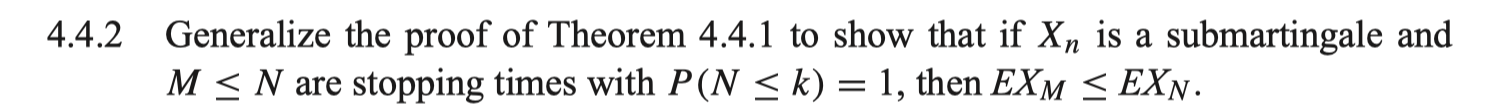
\includegraphics[width=17cm]{Exer4.4.2.png}
\begin{proof}
    Define $K_n=I(M<n\leq N)\foranyn$ . Then $K_n$ is predictable since $$(K_n=1)=(N\geq n)\intersect (M<n)=(N\leq n-1)^C\intersect (M\leq n-1)\in \F_{n-1} $$
    Then, we can define a process $(K\cdot X)_n$ as below :
    \begin{align*}
        (K\cdot X)_n &= \sum_{j=1}^n K_j(X_j-X_{j-1})=\sum_{j=1}^n I(M<j\leq N)(X_j-X_{j-1}) \\ &=\sum_{j=1}^n I(M+1\leq j\leq N)(X_j-X_{j-1}) \\ 
        &= \sum_{j=(M\wedge n)+1}^{N\wedge n} X_j - X_{j-1} = X_{N\wedge n} - X_{M\wedge n} \quad \foranyn
    \end{align*}
    Define $(K\cdot X)_0=0$ . Then since $X_n$ is a submartingale and $K_n$ is a predictable sequence, \\$\{K\cdot X\}_{n\in \N\union \{0\}}$ is a submartingale. It implies that $\{X_{N\wedge n}-X_{M\wedge n}\}_{n\in \N\union\{0\}}$ is a submartingale. \\ Note that if $Y_n$ is a martingale then $E[Y_i]\leq E[Y_j]$ whenever $i\leq j$. Plugging in $i=0$ and $j=k$ on $X_{N\wedge n}-X_{M\wedge n}$ , we have $E[X_0-X_0]\leq E[X_N-X_M]$ since $M\leq N\leq k\;\,a.s.$ . Therefore, $0\leq E[X_N]-E[X_M]$ \;i.e.\; $E[X_N]\geq E[X_M]$
\end{proof}
\vspace{1cm}

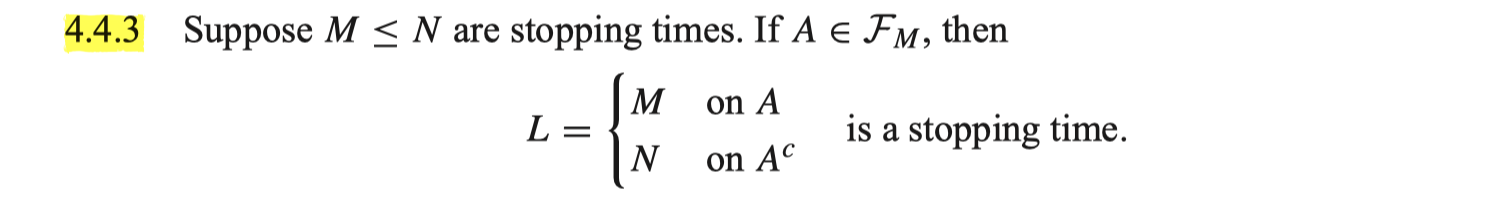
\includegraphics[width=17cm]{Exer4.4.3.png}
\begin{proof}
    $\F_M=\{A\in \F : A\intersect (M=n)\in \F_n \foranyn\}$ . Take $A\in \F_M$ and define $L$ as above. Choose arbitrary $n\in N$ . We want to show that $(L=n)\in \F_n$ . Note that $$(L=n)=\big((M=n)\intersect A\big)\bigcup \big((N=n)\intersect A^C\big)$$
    Since $A\in \F_M$ , $(M=n)\intersect A\in \F_n$ by definition of $\F_M$ . \\ Observe that since $M\leq N$ , $(N=n)=(N=n)\intersect (M\leq N)$ . Using this equality, we get
    \begin{align*}
        (N=n)\intersect A^C&= (N=n)\intersect (M\leq n) \intersect A^C \\
        &= (N=n) \intersect \Big(\bigcup_{k=1}^n \{(M=k)\intersect A^C \}\Big)
    \end{align*}
    Since $A\in \F_M$ and $\F_M$ is a $\sigma$-field , we have $A^C\in \F_M$ so that $(M=k)\intersect A^C\in \F_k\quad \forall\; k\in \N$ . Therefore $\bigcup_{k=1}^n \{(M=k)\intersect A^C \}\in \F_n$. Also, since $N$ is a stopping time , $(N=n)\in \F_n$ \\ Thus $(N=n)\intersect A^C\in \F_n$ and combining with $(M=n)\intersect A\in \F_n$ , we have $(L=n)\in \F_n$
\end{proof}
\clearpage

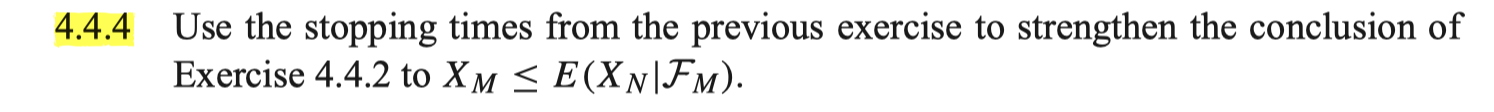
\includegraphics[width=17cm]{Exer4.4.4.png}
\begin{proof}
    Assume $X_n$ is a submartingale and $M\leq N$ are stopping times with $N\leq k\;\,a.s.$ \\ Note that $X_M\in \F_M$ by definition of $\F_M$ and $E[X_N|\F_M]\in \F_M$ by definition of conditional expectation . Hence, if we can show $$\int_A X_M\, dP\leq \int_A E[X_N|\F_M]\, dP \quad \forall \; A\in \F_M$$ then $X_M\leq E[X_N|\F_M]$ is proved. Notice that for $A\in \F_M$ , we have $\int_A E[X_N|\F_M]\, dP=\int_A X_N\, dP$ \\ Thus, it suffices to show that $$\int_A X_M\,dP\leq \int_A X_N\, dP\quad \forall\; A\in \F_M \quad \cdots (*)$$
    Take $A\in \F_M$ . To use the result of the previous exercise, define $L$ by $$L=M\cdot I_A + N\cdot I_{A^C} $$ 
    By Exer. 4.4.3 , $L$ is a stopping time. Notice that $L\leq N$ since $M\leq N$ . Using Exer. 4.4.2 , we have $E[X_L]\leq E[X_N]$ . By the definition of $L$, we have 
    \begin{align*}
        &X_L=X_MI_A+X_NI_{A^C} \\
        &E[X_L] = E[X_MI_A]+E[X_NI_{A^C}] \\
        &E[X_N] = E[X_NI_A]+E[X_NI_{A^C}] \\
        &E[X_MI_A]+E[X_NI_{A^C}]\leq E[X_NI_A]+E[X_NI_{A^C}] \quad \because \; E[X_L]\leq E[X_N] \\
        &E[X_MI_A]\leq E[X_NI_A] \quad \text{i.e.} \quad \int_A X_M\,dP\leq \int_A X_N\, dP
    \end{align*}
    Hence, we have proved $(*)$ holds true. We can conclude that $X_M\leq E[X_N|\F_M]$
\end{proof}
\vspace{1cm}

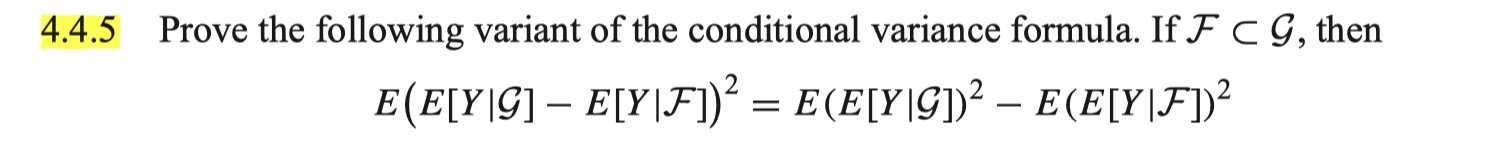
\includegraphics[width=17cm]{Exer4.4.5.png}
\begin{proof}
    We shall take advantage of the fact that for any integrable r.v. $X$ and a $\sigma$-field $\F$ , we have $E[E[X|\F]]=E[X]$ . Also, we will denote $E^2[X]:=\{E(X)\}^2$
    \begin{align*}
        &E\big[\big(E[Y|\G]-E[Y|\F] \big)^2\big] = E\Big[E\big[\big(E[Y|\G]-E[Y|\F] \big)^2 |\F\big]\Big]=E[Z] \\ &\text{where}\quad Z:=E\big[\big(E[Y|\G]-E[Y|\F] \big)^2 |\F\big]=E[W|\F] \\ &\text{with} \quad W:=\big(E[Y|\G]-E[Y|\F] \big)^2\\
        &W=E^2[Y|\G]+E^2[Y|\F]-2E[Y|\G]E[Y|\F] \\
        &\star \text{We shall take }\; E[\;\cdot\;|\F]\\
        &E[E^2[Y|\F]|\F]=E^2[Y|\F]\quad \because\; E^2[Y|\F]\in \F \\
        &E\big[E[Y|\G]E[Y|\F]|\F\big]=E[Y|\F]E\big[E[Y|\G]|\F\big] = E[Y|\F]E[Y|\F] \quad \because\; \F\subset \G \\
        &\Rightarrow\; Z=E[W|\F]= E\big[E^2[Y|\G]|\F \big]+E^2[Y|\F]-2E^2[Y|\F]=E\big[E^2[Y|\G]|\F \big]-E^2[Y|\F] \\
        &E[Z] = E\Big[E\big[E^2[Y|\G]|\F \big]\Big]-E\big[E^2[Y|\F]\big]=E\big[E^2[Y|\G]\big] -E\big[E^2[Y|\F] \big]
    \end{align*}
    Since $E\big[\big(E[Y|\G]-E[Y|\F] \big)^2\big]=E[Z]$ , we have $$E\big[\big(E[Y|\G]-E[Y|\F] \big)^2\big]=E\big[E^2[Y|\G]\big] -E\big[E^2[Y|\F] \big]$$
\end{proof}
\vspace{1cm}

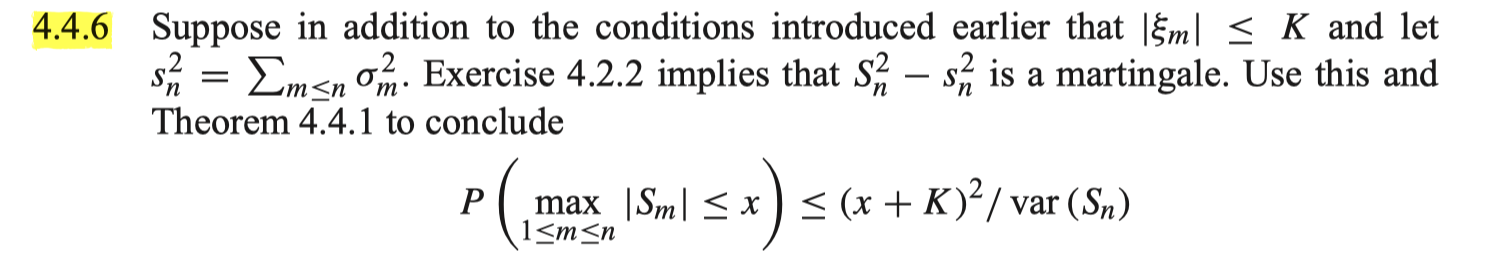
\includegraphics[width=17cm]{Exer4.4.6.png}
\begin{proof}
    Let $\{\xi_n\}_{n\in\N}$ be independent random seq. with $E[\xi_i]=0$ and $E[\xi_i^2]=\sigma_i^2<\infty\quad \forall\;i\in \N$ \\ $S_n, \F_n$ and $s_n^2$ are defined by $S_n=\xi_1+\cdots +\xi_n\;,\; \F_n=\sigma(\xi_1, \cdots, \xi_n)$ and $s_n^2=Var(S_n)=\sum_{i=1}^n \sigma_i^2$ \\Especially, $S_0=0, s_0^2=0$ and $\F_0=\{\phi, \Omega\}$ . In addition, assume $|\xi_n|\leq K\foranyn$ for some $K>0$ \\ Note that $S_n$ is integrable and $S_n\in\F_n$ . Since $s_n^2$ is finite constant for each $n\in\N$ , we have $S_n^2-s_n^2$ is integrable and $S_n^2-s_n^2\in \F_n$ . To show $S_n^2-s_n^2$ is a martingale , it suffices to show that $E[S_{n+1}^2-s_{n+1}^2|\F_n]=S_n^2-s_n^2$ . 
    \begin{align*}
        E[S_{n+1}^2-s_{n+1}^2|\F_n]&= E[(S_n+\xi_{n+1})^2-s_n^2-\sigma_{n+1}^2|\F_n] = E[S_n^2-s_n^2+\xi_{n+1}^2-\sigma_{n+1}^2+2S_n\xi_{n+1}|\F_n] \\
        &= S_n^2-s_n^2+E[\xi_{n+1}^2-\sigma_{n+1}^2]+2S_nE[\xi_{n+1}] = S_n^2-s_n^2
    \end{align*}
    Take $x>0$ . Define $A:=\big(\max_{1\leq m \leq n}|S_m|>x\big)$ . Note that we want to find the upper bound of $P(A^C)$ in this problem. Let $N=\inf\{m\in \N : |S_m|>x\}$ . $N$ is a stopping time since $$(N=n)=(|S_1|\leq x)\intersect \cdots \intersect (|S_{n-1}|\leq x)\intersect (|S_n|>x)\in \F_n \foranyn$$
    Due to the fact that $S_n^2-s_n^2$ is a martingale and $N$ is a stopping time , we have $S_{N\wedge n}^2-s_{N\wedge n}^2$ is also a martingale. Since $N\wedge n\leq n$ , we can apply bounded optional stopping theorem. $$E[S_0^2-s_0^2]=E[S_{N\wedge n}^2-s_{N\wedge n}^2]=E[S_n^2-s_n^2] $$ We will use the left equality, which implies that $E[S_{N\wedge n}^2-s_{N\wedge n}^2]=0\quad \cdots (*)$
    \begin{enumerate}
        \item On $A=\big(\max_{1\leq m \leq n}|S_m|>x\big)$ \\ $|S_m|>x$ for some $m\in \{1,\cdots, n\}$ so that $N\leq n\;\Rightarrow \; N\wedge n=N$ \\ $|S_{N\wedge n}|=|S_N|=|S_{N-1}+\xi_N|\leq |S_{N-1}|+|\xi_N|\leq x+K$
        \item On $A^c=\big(\max_{1\leq m \leq n}|S_m|\leq x\big)$ \\ $|S_m|>x$ is not attined for all $m\in \{1, \cdots, n\}$ so that $N>n\; \Rightarrow N\wedge n =n$ \\ $|S_{N\wedge n}|=|S_n|\leq x$
    \end{enumerate}
    Using $(*)$ , we have the following results.
    \begin{align*}
        &0 = E[S_{N\wedge n}^2-s_{N\wedge n}^2]=E[S_{N\wedge n}^2 I_A+S_{N\wedge n}^2 I_{A^C}]-E[s_{N\wedge n}^2 I_A +s_{N\wedge n}^2 I_{A^C}] \\
        &E[S_{N\wedge n}^2 I_A]\leq E[(x+K)^2 I_A]=(x+K)^2 P(A) \\
        &E[S_{N\wedge n}^2 I_{A^C}]\leq E[x^2 I_{A^C}]=x^2P(A^C) \\
        &E[s_{N\wedge n}^2 I_A]=E[s_N^2 I_A]\geq 0 \quad \surd\; s_N^2 \; \text{is random ; not constant}\\
        &E[s_{N\wedge n}^2 I_{A^C}]=E[s_n^2 I_{A^C}]=s_n^2 P(A^C)=Var(S_n)P(A^C) \\
        &\Rightarrow \; 0 = E[S_{N\wedge n}^2-s_{N\wedge n}^2] \leq (x+K)^2P(A)+x^2P(A^C)-Var(S_n)P(A^C) \\
        &\Rightarrow 0\leq (x+K)^2 - \{Var(S_n)+(x+K)^2-x^2\}P(A^C) \\
        &\Rightarrow (x+K)^2\geq \{Var(S_n)+(x+K)^2-x^2\}P(A^C)\geq Var(S_n)P(A^C)\\
        &\therefore\; P(A^C) \leq \frac{(x+K)^2}{Var(S_n)}
    \end{align*}
    Since $A^C=\big(\max_{1\leq m \leq n}|S_m|\leq x\big)$ , we have proved our desired result.
\end{proof}


\end{document}